\documentclass[T4paper.tex]{subfiles}

\begin{document}
\begin{figure}[!ht]
   \frame{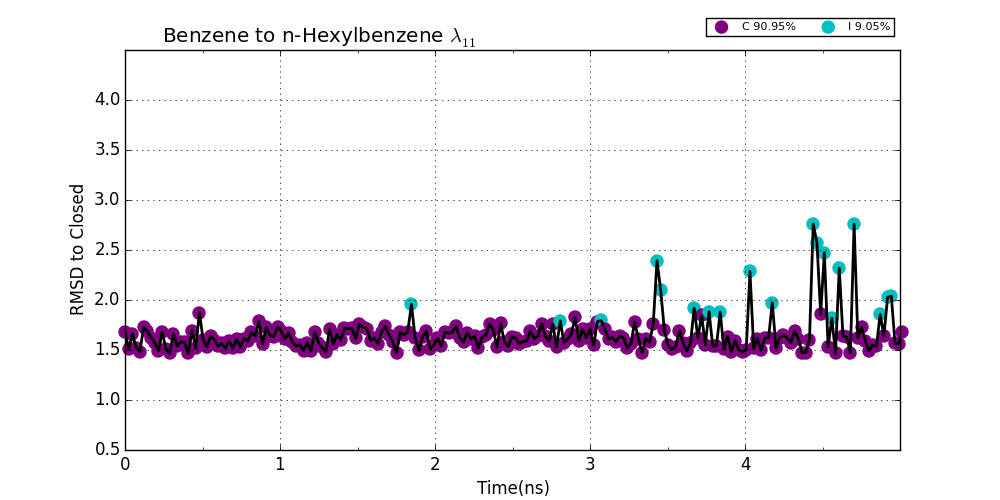
\includegraphics[trim={1.5cm 0 2cm 0.25cm}, clip, width=\textwidth,height=8cm]{VMDscripts/c_opls3_1/plots/0-5ns/RMSD-replica11.png}}
   \caption{Closed - Benzene to n-Hexylbenzene 0-5ns RMSD Replica11}
   \label{fig:c_opls3_1/RMSD-replica11}
\end{figure}

\begin{figure}[!h]
   \frame{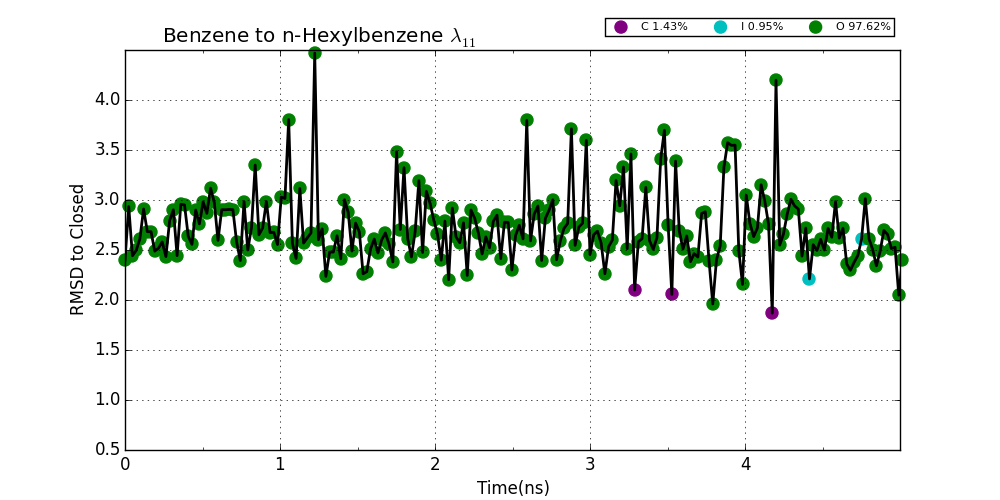
\includegraphics[trim={1.5cm 0 2cm 0.25cm}, clip, width=\textwidth,height=8cm]{VMDscripts/o_opls3_1/plots/0-5ns/RMSD-replica11.png}}
   \caption{Open - Benzene to n-Hexylbenzene 0-5ns RMSD Replica11}
   \label{fig:o_opls3_1/RMSD-replica11}
\end{figure}

\begin{figure}[!h]
   \frame{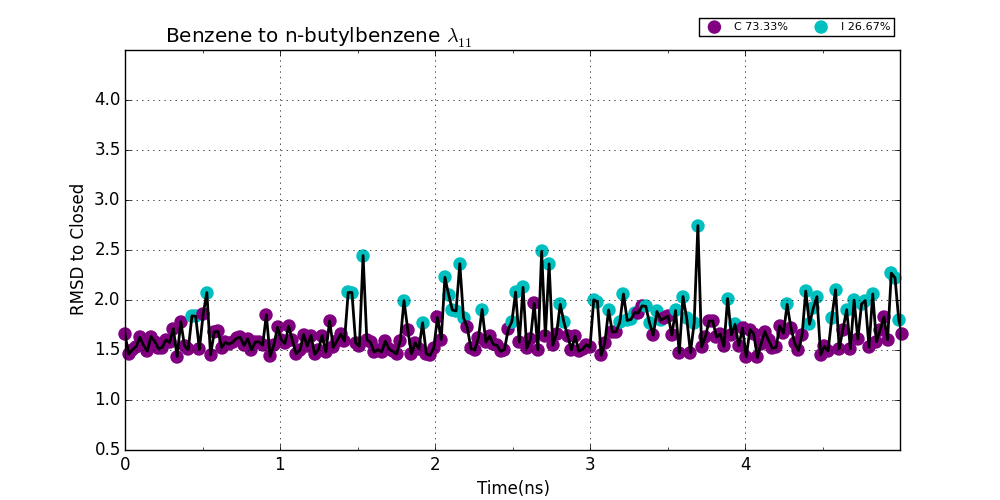
\includegraphics[trim={1.5cm 0 2cm 0.25cm}, clip, width=\textwidth,height=8cm]{VMDscripts/c_exp_opls3_11/plots/0-5ns/RMSD-replica11.png}}
   \caption{Closed - Benzene to n-butylbenzene 0-5ns RMSD Replica11}
   \label{fig:c_exp_opls3_11/RMSD-replica11}
\end{figure}

\begin{figure}[!h]
   \frame{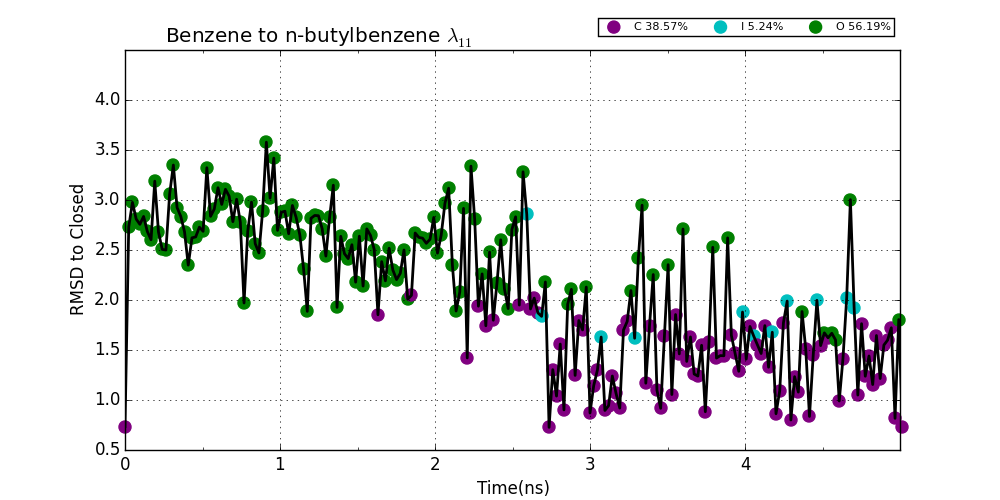
\includegraphics[trim={1.5cm 0 2cm 0.25cm}, clip, width=\textwidth,height=8cm]{VMDscripts/o_exp_opls3_24/plots/0-5ns/RMSD-replica11.png}}
   \caption{Open - Benzene to n-butylbenzene 0-5ns RMSD Replica11}
   \label{fig:o_exp_opls3_24/RMSD-replica11}
\end{figure}

\begin{figure}[!ht]
   \frame{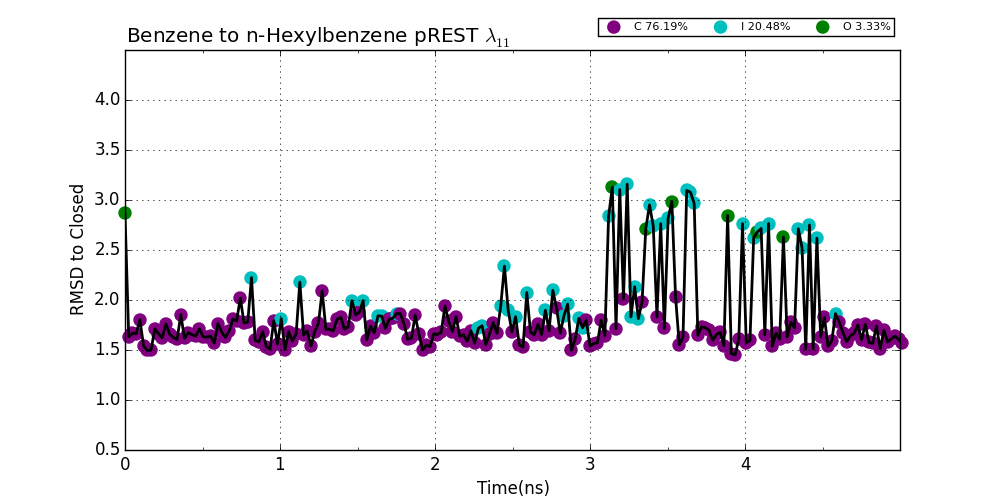
\includegraphics[trim={1.5cm 0 2cm 0.25cm}, clip, width=\textwidth,height=8cm]{VMDscripts/c_opls3_rest1_extend_1e/plots/0-5ns/RMSD-replica11.png}}
   \caption{Closed - Benzene to n-Hexylbenzene 0-5ns RMSD Replica11 pREST}
   \label{fig:c_opls3_rest1_1/RMSD-replica11}
\end{figure}

\begin{figure}[!ht]
   \frame{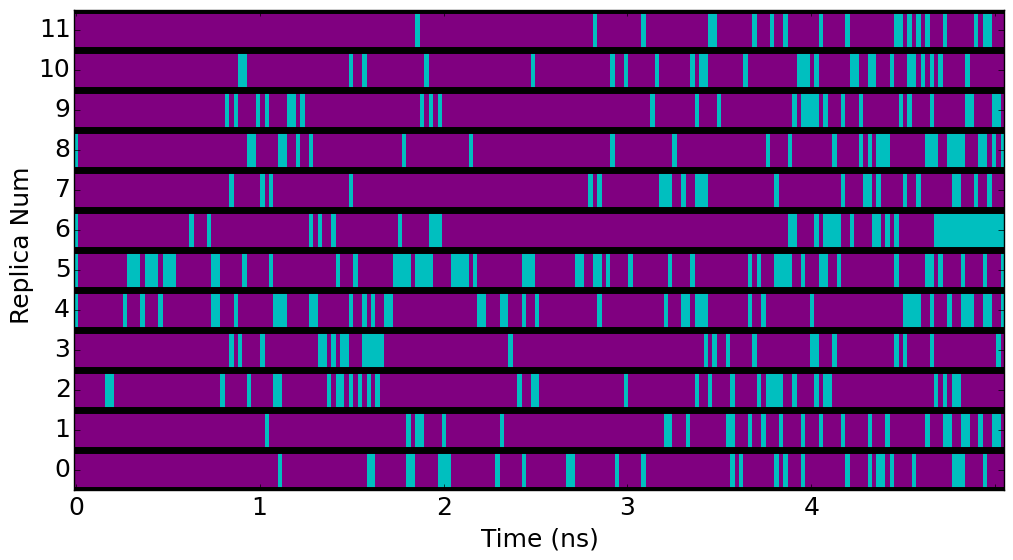
\includegraphics[trim={1.5cm 0 2cm 0.25cm}, clip, width=\textwidth,height=8cm]{VMDscripts/c_opls3_1/plots/colormap/cmap-0-5ns.png}}
   \caption{Closed - Benzene to n-Hexylbenzene 0-5ns Colormap}
   \label{fig:c_opls3_1/colormap}
\end{figure}

\begin{figure}[!ht]
   \frame{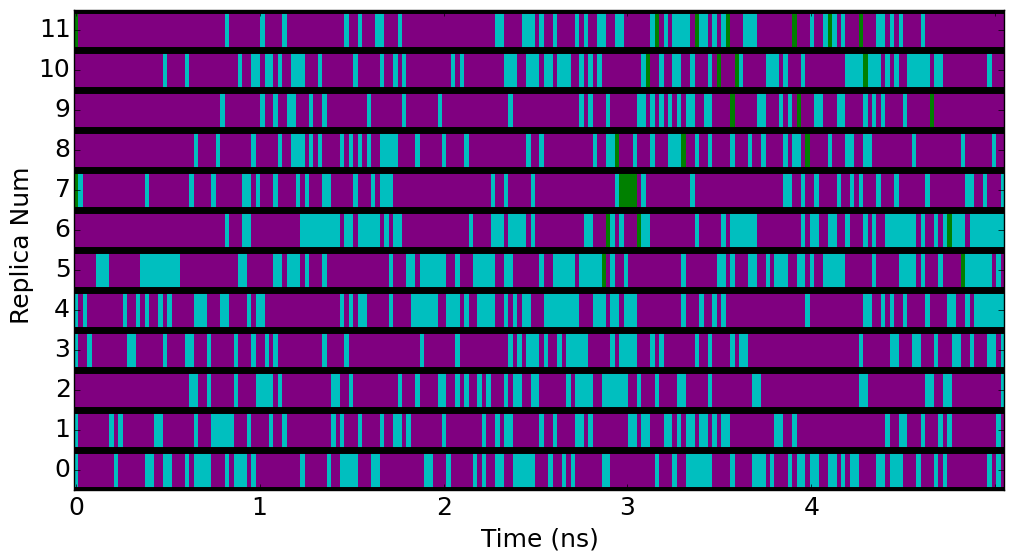
\includegraphics[trim={1.5cm 0 2cm 0.25cm}, clip, width=\textwidth,height=8cm]{VMDscripts/c_opls3_rest1_extend_1e/plots/colormap/cmap-0-5ns.png}}
   \caption{Closed - Benzene to n-Hexylbenzene 0-5ns Colormap pREST}
   \label{fig:c_opls3_rest1_1/colormap}
\end{figure}

\begin{figure}[!ht]
   \frame{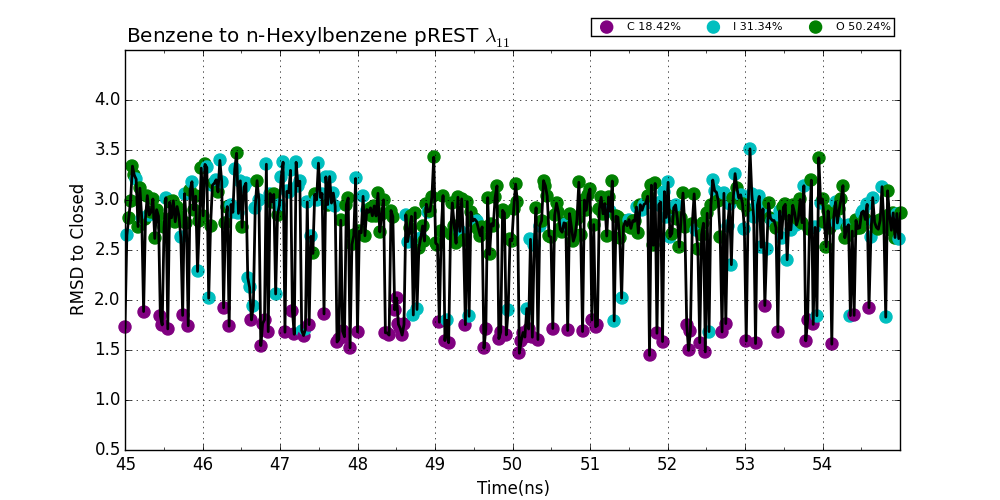
\includegraphics[trim={1.5cm 0 2cm 0.25cm}, clip, width=\textwidth,height=8cm]{VMDscripts/c_opls3_rest1_extend_1e/plots/45-55ns/RMSD-replica11.png}}
   \caption{Closed - Benzene to n-Hexylbenzene 45-55ns RMSD Replica11 pREST}
   \label{fig:c_opls3_rest1_1/45-55ns/RMSD-replica11}
\end{figure}

\begin{figure}[!ht]
   \frame{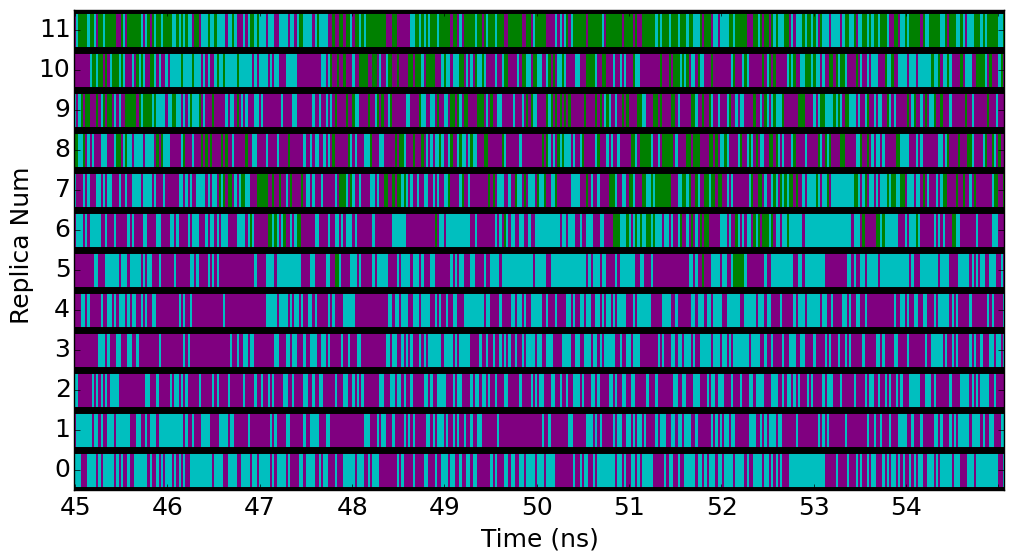
\includegraphics[trim={1.5cm 0 2cm 0.25cm}, clip, width=\textwidth,height=8cm]{VMDscripts/c_opls3_rest1_extend_1e/plots/colormap/cmap-45-55ns.png}}
   \caption{Closed - Benzene to n-Hexylbenzene 45-55ns Colormap pREST}
   \label{fig:c_opls3_rest1_1/cmap-45-55ns}
\end{figure}

\begin{figure}[!ht]
   \frame{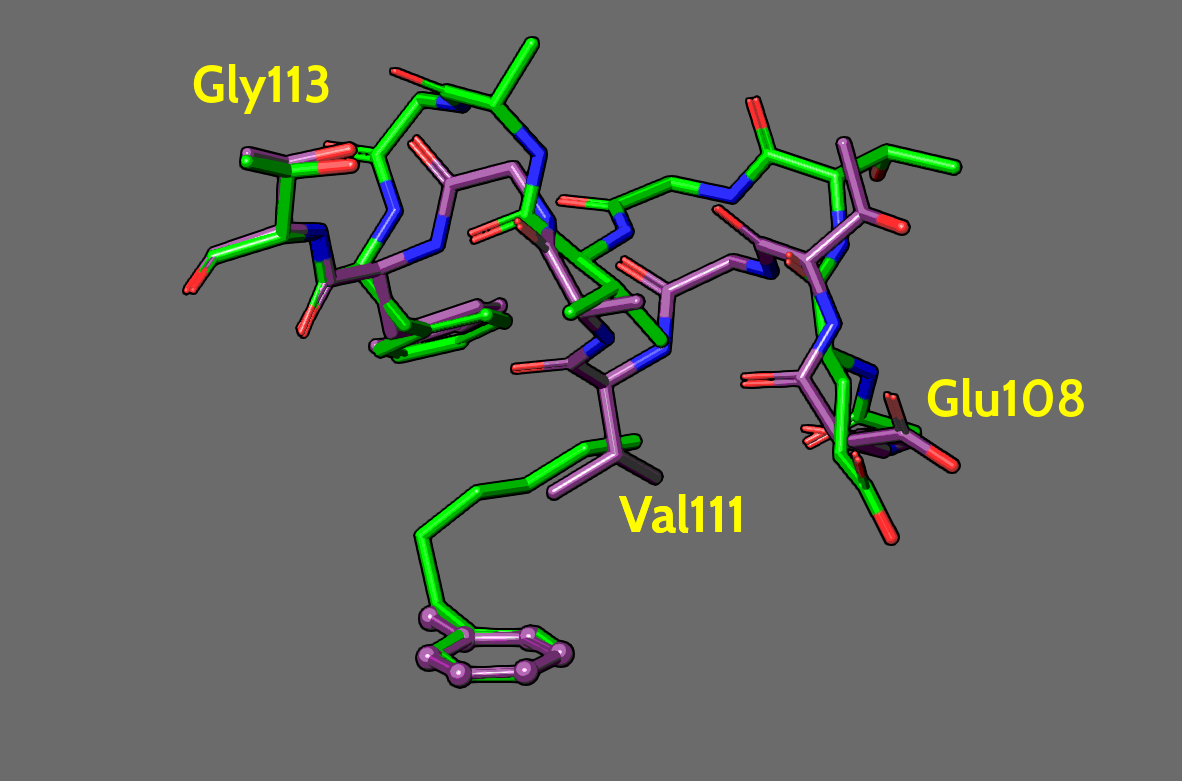
\includegraphics[trim={5cm 2cm 3cm 1cm}, clip, width=\textwidth,height=10cm]{VMDscripts/Figures/C2O.png}}
   \caption{pREST residues}
   \label{fig:C2O}
\end{figure}

\begin{figure}[!ht]
   \frame{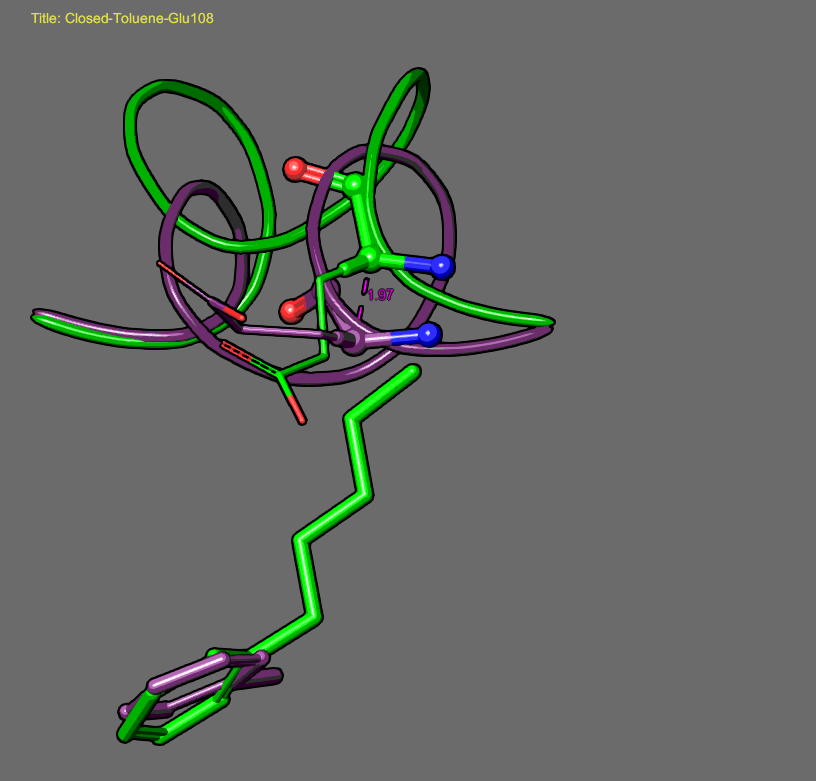
\includegraphics[trim={1cm 1cm 8cm 2cm}, clip, width=\textwidth,height=10cm]{VMDscripts/Figures/Glu108-C2O.png}}
   \caption{Residue Glu108}
   \label{fig:Glu108-C2O}
\end{figure}

\begin{figure}[!ht]
   \frame{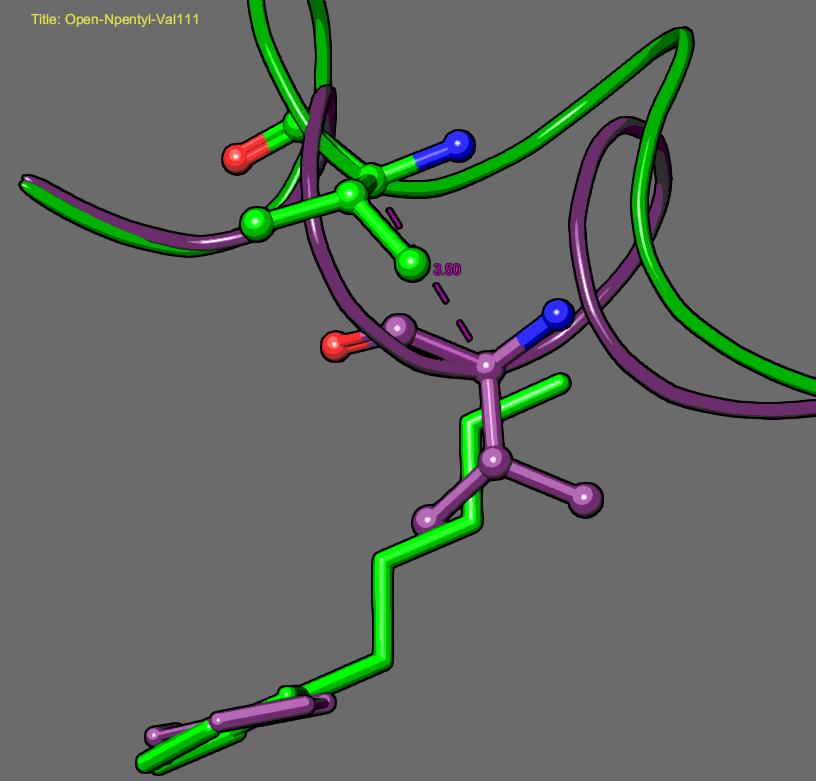
\includegraphics[trim={5cm 0cm 0cm 1cm}, clip, width=\textwidth,height=10cm]{VMDscripts/Figures/Val111-C2O.png}}
   \caption{Residue Val111}
   \label{fig:Val111-C2O}
\end{figure}
\end{document}